\documentclass[11pt,a4paper]{article}

% ==============================================================================
% PACKAGES & CONFIGURATION
% ==============================================================================
\usepackage[utf8]{inputenc}
\usepackage[T1]{fontenc}
\usepackage{lmodern}
\usepackage[margin=1in,headheight=14pt]{geometry}
\usepackage{xcolor}
\usepackage{hyperref}
\usepackage{booktabs}
\usepackage{tabularx}
\usepackage{longtable}
\usepackage{multirow}
\usepackage{amsmath,amssymb,amsfonts}
\usepackage{fancyhdr}
\usepackage{titlesec}
\usepackage{enumitem}
\usepackage{tikz}
\usetikzlibrary{shapes.geometric, arrows, positioning, fit, calc}
\usepackage{tcolorbox}
\tcbuselibrary{skins,breakable}
\usepackage{float}
\usepackage{seqsplit}

% ==============================================================================
% COLOR PALETTE (Corporate Tech Theme)
% ==============================================================================
\definecolor{DeepNavy}{HTML}{1B365D}
\definecolor{SlateBlue}{HTML}{2B547E}
\definecolor{LightSlate}{HTML}{4A607A}
\definecolor{Charcoal}{HTML}{333333}
\definecolor{LightGray}{HTML}{F8FAFC}
\definecolor{BorderGray}{HTML}{D0D7DE}
\definecolor{AccentGreen}{HTML}{1A7F37}
\definecolor{CodeBg}{HTML}{F6F8FA}

% ==============================================================================
% HYPERREF SETUP
% ==============================================================================
\hypersetup{
    colorlinks=true,
    linkcolor=DeepNavy,
    citecolor=SlateBlue,
    urlcolor=SlateBlue,
    pdftitle={DA5402W MLOps Project Report},
    pdfauthor={MLOps Project Team},
    pdfsubject={End-to-End Enterprise MLOps Platform for E-Commerce Recommendation and Churn Prevention}
}

% ==============================================================================
% TYPOGRAPHY & HEADINGS FORMATTING
% ==============================================================================
\titleformat{\section}
  {\color{DeepNavy}\normalfont\Large\bfseries}{\thesection}{1em}{}[\titlerule]
\titleformat{\subsection}
  {\color{SlateBlue}\normalfont\large\bfseries}{\thesubsection}{1em}{}
\titleformat{\subsubsection}
  {\color{LightSlate}\normalfont\normalsize\bfseries}{\thesubsubsection}{1em}{}

\setlist[itemize]{leftmargin=1.5em, itemsep=2pt, topsep=3pt}
\setlist[enumerate]{leftmargin=1.5em, itemsep=2pt, topsep=3pt}

% ==============================================================================
% HEADER & FOOTER CONFIGURATION
% ==============================================================================
\pagestyle{fancy}
\fancyhf{}
\fancyhead[L]{\textcolor{gray}{\small\textit{DA5402W MLOps Project Report}}}
\fancyhead[R]{\textcolor{gray}{\small\textit{Enterprise E-Commerce MLOps Platform}}}
\fancyfoot[L]{\textcolor{gray}{\small\textit{DA5402W-MLOPS-Project}}}
\fancyfoot[R]{\thepage}
\renewcommand{\headrulewidth}{0.4pt}
\renewcommand{\footrulewidth}{0.4pt}

% ==============================================================================
% CUSTOM CALLOUT BOXES
% ==============================================================================
\newtcolorbox{calloutbox}[2][]{
  enhanced,
  colback=LightGray,
  colframe=DeepNavy,
  leftrule=4pt,
  rightrule=0pt,
  toprule=0pt,
  bottomrule=0pt,
  arc=0mm,
  title=\textbf{#2},
  coltitle=DeepNavy,
  fonttitle=\bfseries\sffamily\small,
  attach title to upper={\par\vspace{2pt}},
  boxsep=4pt,
  left=8pt,
  right=8pt,
  top=6pt,
  bottom=6pt,
  #1
}

% ==============================================================================
% DOCUMENT BEGIN
% ==============================================================================
\begin{document}

% ==============================================================================
% TITLE & METADATA BLOCK
% ==============================================================================
\begin{center}
    {\Huge \textbf{\color{DeepNavy} <Title>}} \\[0.8em]
    {\large \textit{\color{SlateBlue} A Scalable, Event-Driven ML Life cycle management for recommendation engine and churn prediction Leveraging Apache Kafka,Spark Streaming for event handling, Airflow & MLflow for model lifecycle management,FastAPI for Model Serving, Prometheus/Grafana for Observability, and Jenkins for CI/CD}} \\[1.2em]
    \rule{\textwidth}{1pt}
\end{center}

\vspace{-0.5em}


\begin{calloutbox}{EXECUTIVE SUMMARY}
This technical report presents the architectural design, ML Lifecycle management, operational orchestration, automated deployment, and continuous monitoring of an MLOps platform engineered for ecommerce usecase. The platform simultaneously serves real-time basket cross-sell recommendations  and intercepts real-time cart abandonments for targeted retention discounts via distributed streaming analytics and closed-loop ML governance.
\end{calloutbox}

% ==============================================================================
% 1. PROBLEM STATEMENT
% ==============================================================================
\section{Problem Statement}

Users journey in an ecommerce platform before becoming a customer(final transacted user) involves browsing for interested products,Shortlisting and adding products to carts and finally checking out and paying. Successful conversion of users to customers requires make the UX frictionless. Two main areas which improves user-conversion rate is recommending users accurately and quickly to reduce user-effort to find required products and find high churn stages where user drops out more and taking preemptive steps. Also Modern digital commerce ecosystems operate under demanding concurrency requirements, where millions of concurrent user interactions generate massive clickstream events every minute. To sustain competitive conversion rates and customer lifetime value (LTV), e-commerce platforms must deliver immediate, context-aware personalized product recommendations while simultaneously mitigating customer churn and cart abandonment in real time. Also these two systems has to be actively retraining to keep updated with minimal developer or human intervention in loop and need active monitoring or observability to keep systems alive at scale.

Traditional machine learning implementations in the retail industry suffer from acute operational bottlenecks:

\begin{itemize}
    \item \textbf{Stale Recommendation Latency:} Standard collaborative filtering and deep neural recommender architectures require intensive matrix factorizations or graph computations that are typically recalculated in overnight batch cycles. Consequently, newly added items, transient session trends, and real-time cart combinations cannot be dynamically cross-sold within active shopper sessions.
    \item \textbf{Delayed Cart Abandonment Recovery:} Industry benchmarks indicate that over 68\% to 75\% of e-commerce shopping carts are abandoned before checkout completion. Traditional analytics platforms detect customer drop-off days or weeks after the session through batch reports, missing the narrow time window (typically 15 to 30 minutes) during which proactive engagement (e.g., targeted discount incentives) can recover the transaction.
    
    \item \textbf{Absence of Real-Time Business Analytics:} Business stakeholders (merchandising, marketing, and operations teams) need up-to-date visibility into funnel drop-off rates, recommendation click-through, and refund/return volumes to steer promotions and inventory decisions. When these KPIs are only available through manual SQL queries or next-day batch reports, decisions lag behind actual customer behavior by hours or days, making it impossible to react to in-session trends such as a sudden spike in cart abandonment for a specific category.
    
    \item \textbf{Fragmented MLOps Governance and Operational Telemetry:} ML models frequently fail in production due to unmonitored data distribution shift, unversioned training pipelines, manual error-prone deployment procedures, and absence of unified service-level observability across data pipelines, streaming consumers, and REST serving endpoints.
\end{itemize}

To resolve these challenges, we demonstrate a unified, closed-loop MLOps architecture that bridges continuous clickstream streaming, automated distributed ETL, dual-model training pipelines (Apriori Market Basket Mining and Random Forest Customer Value Scoring), dynamic MLflow model registry promotion, sub-ms REST inference microservices, Online analytics and end-to-end Prometheus/Grafana observability.

\begin{calloutbox}{CORE OPERATIONAL TARGETS \& SLA CONTRACTS}
\begin{itemize}
    \item \textbf{Real-Time Recommendation SLA:} Deliver cross-sell recommendations within milliseconds per request via containerized FastAPI inference.
    \item \textbf{Cart Abandonment Interception SLA:} Detect abandoned user sessions within 60 seconds of a 15-minute inactivity window and simulate personalized tiered incentives.
    \item \textbf{Continuous Automated Retraining:} Orchestrate daily batch retraining and DVC data pushes via scheduled Apache Airflow DAGs.
    \item \textbf{Automated Quality Gate:} Zero-downtime model promotion in MLflow based on strict validation thresholds without requiring server restarts.
    \item \textbf{Comprehensive Observability:} 100\% telemetry scraping across all 11 microservice containers via Prometheus and Grafana.
    \item \textbf{Daily Business Analytics:} Compute and persist funnel, recommendation-CTR, and refund KPIs once per day via the Airflow-orchestrated analytics job, so business stakeholders always have a same-day view of platform health.
\end{itemize}
\end{calloutbox}

% ==============================================================================
% 2. DATASET DESCRIPTION
% ==============================================================================
\section{Dataset Description}

The platform processes a hybrid data corpus combining extensive real-world product metadata with high-volume, multi-topic synthetic behavioral clickstream streams. This design reflects real-world enterprise architectures where static dimension tables are enriched with continuous, high-throughput user interaction telemetry.

\subsection{Real-World E-Commerce Catalog Data}
The relational product catalog is seeded into PostgreSQL (\texttt{ecommdb}) from curated enterprise e-commerce datasets:

\begin{table}[h]
\centering
\small
\begin{tabularx}{\textwidth}{@{}>{\bfseries}p{3.6cm}p{2.6cm}p{4.2cm}X@{}}
\toprule
\color{DeepNavy}Dataset / File & \color{DeepNavy}Volume / Size & \color{DeepNavy}Primary Attributes & \color{DeepNavy}Schema \& Pipeline Functionality \\
\midrule
\texttt{amazon\_products.csv} & 375.9 MB ($\sim$1.4M rows) & \texttt{id, title, category\_id, price, image\_url, rating} & Master product inventory used for search, cart browsing, and candidate lookup. \\
\addlinespace
\texttt{amazon\_categories.csv} & 7.1 KB (250 rows) & \texttt{id, category\_name, parent\_id} & Hierarchical taxonomy mapping for multi-level category navigation. \\
\addlinespace
\texttt{users.csv} & 482 B (Seed users) & \texttt{id, email, password\_hash, created\_at} & Baseline authenticated profiles supporting auth, sessions, and purchase linkage. \\
\addlinespace
\texttt{events.csv} (Baseline) & 20.2 MB ($\sim$275K rows) & \texttt{id, session\_id, user\_id, timestamp, event\_type, product\_id} & Historical interaction log used for initial cold-start training of Apriori and churn baselines. \\
\bottomrule
\end{tabularx}
\caption{Real-World Reference Catalog and Historical Event Corpora}
\end{table}

\subsection{Real-Time Event Stream Taxonomy \& Schema Specification}
The streaming infrastructure utilises three partitioned Apache Kafka topics, segregating interaction types to optimize consumer throughput:

\begin{table}[h]
\centering
\small
\begin{tabularx}{\textwidth}{@{}>{\bfseries}p{3.5cm}p{4.2cm}X@{}}
\toprule
\color{DeepNavy}Kafka Topic & \color{DeepNavy}Event Types Emitted & \color{DeepNavy}Operational \& Business Role \\
\midrule
\texttt{user-events} & \texttt{view, add\_to\_cart, delete\_from\_cart, quantity, transaction, refund\_request} & Tracks primary user interactions, cart mutations, checkout conversions, and post-purchase disputes. \\
\addlinespace
\texttt{recommendation-actions} & \texttt{recommendation\_shown, recommendation\_clicked, recommendation\_accepted, recommendation\_rejected} & Captures user responses to algorithmic recommendations, enabling real-time Click-Through Rate (CTR) and conversion lift analytics. \\
\addlinespace
\texttt{notification-events} & \texttt{discount\_offer\_sent, reminder\_sent, offer\_accepted, offer\_declined} & Tracks churn retention interventions, discount voucher generation, and customer redemption behavior. \\
\bottomrule
\end{tabularx}
\caption{Kafka Multi-Topic Stream Partitioning Architecture}
\end{table}

\subsection{Event Simulation Engine \& Behavioral Modeling}
The synthetic event generator (\texttt{producer.py}, \texttt{eventProducer.py}, and \texttt{launch\_producer.py}) simulates session-consistent e-commerce traffic driven by hidden per-customer behavioral profiles, rather than uniformly random clicks:
\begin{itemize}
    \item \textbf{Hidden Customer Personas:} Each simulated customer is assigned a latent persona (\texttt{assign\_personas()}) comprising a \emph{purchase-intent} score drawn from a right-skewed $\text{Beta}(2,5)$ distribution (most customers are low-intent browsers, a minority convert readily), an \emph{indecisiveness} score drawn from $\text{Beta}(2,2)$ (governing how often a product is re-viewed or added/removed from the cart before a decision), and a categorical \emph{engagement level} (low 50\% / medium 35\% / high 15\%) governing session frequency. This persona table is written to \texttt{customer\_personas.csv} strictly as simulation ground truth for later model evaluation and is never fed into the event stream as a feature.
    \item \textbf{Session-Consistent Funnel Simulation:} On each simulated day, a persona-weighted subset of active users generates a view $\rightarrow$ add-to-cart $\rightarrow$ quantity-adjust $\rightarrow$ transaction/abandon journey. Abandoned carts are queued and followed up with a discount offer or reminder 1--3 days later, producing realistic \texttt{discount\_offer\_sent} / \texttt{reminder\_sent} / \texttt{offer\_accepted} / \texttt{offer\_declined} sequences whose acceptance probability itself scales with the customer's purchase-intent score.
    \item \textbf{Decoupled Streaming Engine:} \texttt{launch\_producer.py} runs the generator in a dedicated child process (via \texttt{multiprocessing} with the \texttt{spawn} start method, so live Kafka socket connections are never inherited across a fork), looping indefinitely to generate and publish continuous batches (default: 500 events every 5 seconds) instead of a single fixed burst.
    \item \textbf{Topic-Aware Publishing:} Every generated event is tagged with its target Kafka topic (\texttt{user-events}, \texttt{recommendation-actions}, or \texttt{notification-events}) and published via \texttt{KafkaProducer.send(topic, record)}. Topics are pre-provisioned with 3 partitions each by a one-shot \texttt{topic-init} container, which \texttt{event-producer} depends on via a \texttt{service\_completed\_successfully} condition so no events are ever sent before the topics exist.
\end{itemize}

\newpage
% ==============================================================================
% 3. SYSTEM ARCHITECTURE
% ==============================================================================
\section{System Architecture}

The platform is designed as a distributed, decoupled microservices architecture containerized through Docker Compose. All components operate within a shared bridge network (\texttt{spark-kafka-net}), enabling seamless inter-service DNS resolution, low-latency internal communication, and isolated failure domains.

\subsection{Component Topology \& Microservices Breakdown}

\begin{table}[h]
\centering
\scriptsize
\begin{tabularx}{\textwidth}{@{}>{\bfseries}p{2.8cm}p{2.3cm}p{2.2cm}p{2.8cm}X@{}}
\toprule
\color{DeepNavy}Service Identifier & \color{DeepNavy}Container & \color{DeepNavy}Port Mappings & \color{DeepNavy}Tech Stack & \color{DeepNavy}Primary Responsibility \\
\midrule
Kafka Broker & \texttt{kafka} & 9094, 7071 (JMX) & Apache Kafka 3.7.0 & Event streaming backbone for clickstream and notifications. \\
Topic Initializer & \texttt{topic-init} & Internal & Kafka CLI, Bash & Idempotent topic provisioning container on broker startup. \\
Event Producer & \texttt{event-producer} & Internal & Python 3.10, NumPy & Continuous synthetic traffic generator. \\
Spark Consumer & \texttt{spark-consumer} & Internal & PySpark, Kafka JAR & Streaming consumer demuxing streams into Parquet dumps. \\
Spark Master / Mon & \texttt{spark-master} & 4040, 9090, 3000 & Spark 3.5, Prom, Graf & Manages cluster resources and co-hosts monitoring servers. \\
Airflow Orchestrator & \texttt{airflow-webserver} \newline \texttt{airflow-scheduler} & 8080 (UI), \newline 9091 (StatsD) & Airflow 2.8, \newline LocalExecutor & Orchestrates batch ETL, feature engineering, and DVC sync. \\
Airflow Metadata DB & \texttt{airflow-postgres} & 5432:5432 & PostgreSQL 13 & Relational store for Airflow task execution states and locks. \\
MLflow Registry & \texttt{mlflow} & 5000:5000 & MLflow Server & Tracks runs, parameters, metrics, and manages \texttt{@champion}. \\
MLflow Metadata DB & \texttt{mlflow-postgres} & 5434:5432 & PostgreSQL 13 & Backend database storing MLflow experiments and registry data. \\
E-Comm Backend & \texttt{ecomm-backend} & 5001:5001 & Flask, SQLAlchemy & Core web API for catalog, cart, checkout, and Kafka emit. \\
E-Comm Database & \texttt{ecomm-postgres} & 5433:5432 & PostgreSQL 13 & Relational store for catalog, orders, and discount vouchers. \\
Apriori Recommender & \texttt{apriori-api} & 5002:5002 & FastAPI, Uvicorn & REST microservice serving sub-50ms recommendations. \\
Churn Notifier & \texttt{churn-notifier} & Internal & Python, MLflow & Tracks cart inactivity and dispatches targeted discount incentives. \\
Angular Frontend & \texttt{frontend} & 4200:4200 & Angular 17, RxJS & Single-page shopping application with dynamic recommendation UI. \\
\bottomrule
\end{tabularx}
\caption{System Microservices Architecture Specification}
\end{table}

\subsection{End-to-End Architectural Flow Diagram}
Figure~\ref{fig:arch} illustrates the event streaming, batch training, model registry, inference serving, and monitoring feedback loops.
\begin{figure}[h]
\centering
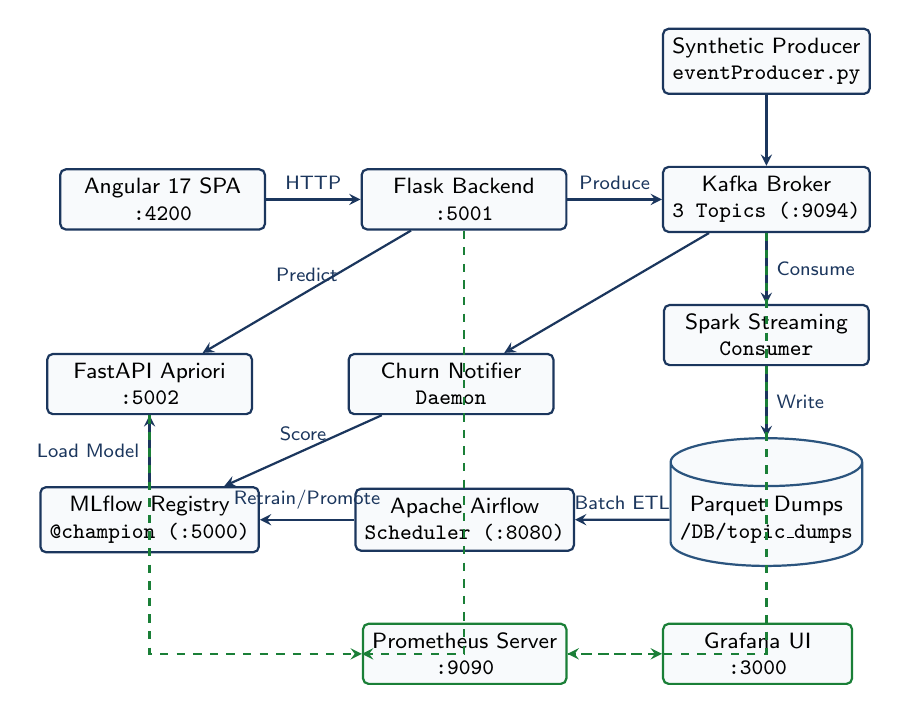
\begin{tikzpicture}[
    node distance=0.9cm and 1.2cm,
    font=\sffamily\footnotesize,
    box/.style={rectangle, draw=DeepNavy, fill=LightGray, rounded corners=2pt, minimum width=2.6cm, minimum height=0.75cm, align=center, line width=0.8pt},
    store/.style={cylinder, draw=SlateBlue, fill=LightGray, shape border rotate=90, aspect=0.25, minimum width=2.4cm, minimum height=0.75cm, align=center, line width=0.8pt},
    mon/.style={rectangle, draw=AccentGreen, fill=LightGray, rounded corners=2pt, minimum width=2.4cm, minimum height=0.75cm, align=center, line width=0.8pt},
    arr/.style={-stealth, thick, color=DeepNavy}
]
    % Ingestion & Frontend
    \node[box] (ui) {Angular 17 SPA \\ \texttt{:4200}};
    \node[box, right=of ui] (backend) {Flask Backend \\ \texttt{:5001}};
    \node[box, right=of backend] (kafka) {Kafka Broker \\ \texttt{3 Topics (:9094)}};
    \node[box, above=of kafka] (producer) {Synthetic Producer \\ \texttt{eventProducer.py}};

    % Streaming & Storage
    \node[box, below=of kafka] (spark) {Spark Streaming \\ \texttt{Consumer}};
    \node[store, below=of spark] (parquet) {Parquet Dumps \\ \texttt{/DB/topic\_dumps}};

    % Orchestration & Registry
    \node[box, left=of parquet] (airflow) {Apache Airflow \\ \texttt{Scheduler (:8080)}};
    \node[box, left=of airflow] (mlflow) {MLflow Registry \\ \texttt{@champion (:5000)}};

    % Inference & Churn
    \node[box, above=of mlflow] (fastapi) {FastAPI Apriori \\ \texttt{:5002}};
    \node[box, right=of fastapi] (churn) {Churn Notifier \\ \texttt{Daemon}};

    % Monitoring
    \node[mon, below=of airflow] (prom) {Prometheus Server \\ \texttt{:9090}};
    \node[mon, right=of prom] (graf) {Grafana UI \\ \texttt{:3000}};

    % Connections
    \draw[arr] (ui) -- node[above]{\scriptsize HTTP} (backend);
    \draw[arr] (backend) -- node[above]{\scriptsize Produce} (kafka);
    \draw[arr] (producer) -- (kafka);
    \draw[arr] (kafka) -- node[right]{\scriptsize Consume} (spark);
    \draw[arr] (spark) -- node[right]{\scriptsize Write} (parquet);
    \draw[arr] (parquet) -- node[above]{\scriptsize Batch ETL} (airflow);
    \draw[arr] (airflow) -- node[above]{\scriptsize Retrain/Promote} (mlflow);
    \draw[arr] (mlflow) -- node[left]{\scriptsize Load Model} (fastapi);
    \draw[arr] (backend) -- node[above]{\scriptsize Predict} (fastapi);
    \draw[arr] (kafka) -- (churn);
    \draw[arr] (churn) -- node[above]{\scriptsize Score} (mlflow);
    \draw[arr, dashed, color=AccentGreen] (prom) -- (graf);
    \draw[arr, dashed, color=AccentGreen] (backend) |- (prom);
    \draw[arr, dashed, color=AccentGreen] (fastapi) |- (prom);
    \draw[arr, dashed, color=AccentGreen] (kafka) |- (prom);
\end{tikzpicture}
\caption{End-to-End Distributed Architecture and Data Interaction Diagram\n<Have to verify architecute diagram as group>}
\label{fig:arch}
\end{figure}

% ==============================================================================
% 4. DATA PIPELINE
% ==============================================================================
\section{Data Pipeline}

The data engineering subsystem encompasses both high-throughput real-time streaming pipelines and deterministic, version-controlled batch ETL workflows.

\subsection{Streaming Ingestion \& Spark Structured Streaming}
The streaming consumer (\texttt{spark\_streaming\_consumer.py}) connects to Kafka using PySpark Structured Streaming with micro-batch triggers:
\begin{itemize}
    \item \textbf{Schema Enforcement:} Enforces rigid typing via \texttt{EVENT\_SCHEMA} (\texttt{id, session\_id, user\_id, timestamp, event\_type, product\_id, is\_recommended}), isolating corrupted payloads into dead-letter sinks.
    \item \textbf{Dynamic Topic Splitting:} Parses incoming JSON streams and routes records to dedicated partitioned Parquet destinations: \texttt{/DB/topic\_dumps/user\_events}, \texttt{/DB/topic\_dumps/recommendation\_events}, and \texttt{/DB/topic\_dumps/notification\_events}.
    \item \textbf{Fault-Tolerant State Checkpointing:} Spark Structured Streaming checkpoints (\texttt{/opt/spark/work-dir/checkpoints}) track offset commits, ensuring exactly-once processing across consumer restarts.
\end{itemize}

\subsection{Batch ETL \& Feature Engineering Pipelines}
Apache Airflow orchestrates batch extraction jobs on daily schedules (\texttt{0 2 * * *}) to transform raw parquet topic dumps into model training matrices:

\begin{table}[h]
\centering
\small
\begin{tabularx}{\textwidth}{@{}>{\bfseries}p{3.5cm}p{3.2cm}p{4.2cm}X@{}}
\toprule
\color{DeepNavy}Pipeline Stage & \color{DeepNavy}Input Source & \color{DeepNavy}Core Transformation Logic & \color{DeepNavy}Output Target \\
\midrule
Spark Batch ETL \newline (\texttt{spark\_etl.py}) & Parquet files in \newline \texttt{/DB/topic\_dumps} & Reads incremental partitions, flattens timestamps, deduplicates events, and exports unified CSV. & \texttt{/DB/events\_from\_kafka.csv} \\
\addlinespace
Apriori Feature Extr. \newline (\texttt{feature.py}) & \texttt{/DB/events\_from\_kafka.csv} & Groups clickstream by session, extracts cart and checkout product lists as JSON arrays. & \texttt{/DB/extracted\_features.csv} \\
\addlinespace
Churn Feature Eng. \newline (\texttt{feature\_churn.py}) & \texttt{/DB/events\_from\_kafka.csv} & Aggregates per-user interaction counts, unique sessions, conversion rates, and abandonment rates. & \texttt{/DB/user\_value\_features.csv} \\
\addlinespace
Daily Analytics \newline (\texttt{analytics.py}) & All topic dumps & Computes business KPIs: active customers, funnel drop-off, CTR on recommendations, and refunds. & \texttt{/DB/analytics/} \\
\bottomrule
\end{tabularx}
\caption{Airflow Batch ETL and Feature Engineering Transformation Matrix}
\end{table}

\subsection{Data Version Control (DVC) Integration}
To ensure end-to-end dataset reproducibility, Data Version Control (DVC) is directly integrated into the Airflow DAG workflows. Every batch ETL execution triggers an automated \texttt{dvc push DB/topic\_dumps.dvc} task. The underlying Parquet data hashes are committed to Git, guaranteeing that any model artifact registered in MLflow can be precisely traced back to the exact snapshot of training data ingested.

% ==============================================================================
% 5. MODEL DEVELOPMENT
% ==============================================================================
\section{Model Development}

The platform houses two distinct machine learning systems engineered for specific operational objectives: an unsupervised association rule engine for basket recommendations and a supervised ensemble classifier for customer lifetime value and churn scoring.

\subsection{Apriori Market Basket Association Recommender}
The recommendation engine (\texttt{train\_model\_apriori.py}) analyzes historical co-purchasing patterns to generate high-affinity cross-sell rules:
\begin{itemize}
    \item \textbf{One-Hot Transaction Encoding:} Baskets extracted from user sessions are transformed into a sparse boolean matrix using \texttt{TransactionEncoder} from \texttt{mlxtend}.
    \item \textbf{Frequent Itemset Discovery:} Evaluates candidate item combinations meeting the support threshold (default $\text{min\_support} = 0.001$).
    \item \textbf{Association Rule Mining Metrics:} Mined itemsets are converted into directional association rules ($A \rightarrow B$) evaluated across standard association metrics:
    \begin{align}
        \text{Support}(A \rightarrow B) &= P(A \cap B) = \frac{\text{Count}(A \cup B)}{\text{Total Baskets}} \\
        \text{Confidence}(A \rightarrow B) &= P(B \mid A) = \frac{\text{Support}(A \cup B)}{\text{Support}(A)} \\
        \text{Lift}(A \rightarrow B) &= \frac{\text{Confidence}(A \rightarrow B)}{\text{Support}(B)} = \frac{P(A \cap B)}{P(A) \cdot P(B)} \\
        \text{Conviction}(A \rightarrow B) &= \frac{1 - \text{Support}(B)}{1 - \text{Confidence}(A \rightarrow B)}
    \end{align}
    \item \textbf{MLflow PyFunc Custom Wrapper (\texttt{apriori\_mlflow\_predict.py}):} Wraps mined association rules in an \texttt{mlflow.pyfunc.PythonModel} class. The inference function accepts input item lists, searches antecedent rule matches, sorts by highest lift, and returns top-$K$ consequent product recommendations.
\end{itemize}

\subsection{Customer Value Scoring \& Churn Classifier}
The churn prediction model (\texttt{train\_churn\_model.py}) categorizes registered customers into three actionable value/risk tiers (0: Low Value/High Churn Risk, 1: Medium Value, 2: High Value/Loyal):

\begin{table}[h]
\centering
\small
\begin{tabularx}{\textwidth}{@{}>{\bfseries}p{3.8cm}p{1.8cm}p{4.5cm}X@{}}
\toprule
\color{DeepNavy}Feature Name & \color{DeepNavy}Data Type & \color{DeepNavy}Calculation Methodology & \color{DeepNavy}Predictive Signal \\
\midrule
\texttt{transaction\_count} & Integer & Total successful transaction events & Monetary value and platform commitment. \\
\texttt{add\_count / remove\_count} & Integer & Total add-to-cart vs. item deletions & Shopping intent vs. purchase indecision. \\
\texttt{conversion\_rate} & Float & $\text{transaction\_count} / \text{add\_count}$ & Checkout funnel progression efficiency. \\
\texttt{cart\_abandon\_rate} & Float & $\text{abandoned\_sessions} / \text{total\_sessions}$ & Primary indicator of drop-off propensity. \\
\texttt{recommendation\_ctr} & Float & $\text{rec\_clicked} / \text{rec\_shown}$ & Algorithmic promotional receptivity. \\
\texttt{days\_since\_last\_tx} & Integer & Snapshot date $-$ last transaction date & Recency component of RFM modeling. \\
\texttt{events\_per\_day / active\_days} & Float / Int & $\text{total\_events} / \text{lifespan}$; active days & Overall engagement and customer loyalty. \\
\bottomrule
\end{tabularx}
\caption{Engineered Behavioral Features for Customer Churn Modeling}
\end{table}

\begin{itemize}
    \item \textbf{Pipeline Architecture:} Scikit-learn \texttt{Pipeline} combining \texttt{StandardScaler()} with a \texttt{RandomForestClassifier(n\_estimators=100, max\_depth=8, class\_weight='balanced')}.
    \item \textbf{Validation Strategy:} 5-fold stratified cross-validation on Macro F1 score:
    \begin{equation}
        \text{F1}_{\text{Macro}} = \frac{1}{|C|} \sum_{c \in C} 2 \cdot \frac{\text{Precision}_c \cdot \text{Recall}_c}{\text{Precision}_c + \text{Recall}_c}
    \end{equation}
    \item \textbf{Explainability:} Gini impurity feature importances are extracted and logged to MLflow on every run.
\end{itemize}

\subsection{Automated MLflow Model Registry \& Champion Gate}
The project implements an automated, metric-driven promotion engine (\texttt{mlflow\_registry.py}). When training completes:
\begin{enumerate}
    \item \textbf{Logging:} All runs log parameters, per-class precision/recall, macro-F1, confusion matrices, and serialized model artifacts to MLflow Tracking Server.
    \item \textbf{Benchmark Comparison:} The \texttt{promote\_if\_best()} function queries MLflow Client for the existing \texttt{@champion} alias version and its recorded primary metric (\texttt{avg\_lift} for Apriori, \texttt{f1\_macro} for Churn).
    \item \textbf{Atomic Promotion:} If the newly trained candidate strictly exceeds the current champion's benchmark, the \texttt{@champion} alias is atomically reassigned to the new version without downtime.
\end{enumerate}

% ==============================================================================
% 6. DEPLOYMENT STRATEGY
% ==============================================================================
\section{Deployment Strategy}

The deployment architecture emphasizes containerization, high availability, zero-downtime hot-swapping of models, and sub-second recovery.

\subsection{Real-Time Model Serving Architecture}
Production inference is decoupled from training infrastructure through specialized serving containers:
\begin{itemize}
    \item \textbf{FastAPI Apriori Recommender (\texttt{apriori\_http\_service.py}):} Built with FastAPI and Uvicorn. On startup (or first request), it dynamically pulls \texttt{models:/AprioriRecommender@champion} from MLflow. Exposes \texttt{/health} and \texttt{/predict} endpoints.
    \item \textbf{Streaming Churn Notifier (\texttt{service-churn-notifier/app.py}):} Persistent daemon subscribing to \texttt{user-events} Kafka topic, tracking in-memory cart states, and executing periodic abandonment scans every 60 seconds.
    \item \textbf{Flask Application Backend (\texttt{service-backend/app.py}):} Serves REST endpoints for authentication, product catalog, cart management, and order fulfillment. Directly proxies recommendation queries to \texttt{http://apriori-api:5002} and publishes interaction events to Kafka.
\end{itemize}

\subsection{Dynamic Model Hot-Reloading}
Because inference services reference the \texttt{@champion} alias rather than static pickle files or hardcoded version IDs, retraining DAGs can promote a superior model in MLflow while serving services automatically fetch and instantiate the new champion on subsequent invocations without requiring container restarts or incurring API downtime.

% ==============================================================================
% 7. MONITORING STRATEGY
% ==============================================================================
\section{Monitoring Strategy}

Comprehensive observability is implemented across all architectural layers using a pull-based Prometheus server coupled with pre-configured Grafana visualization dashboards. Both processes are co-located inside the \texttt{spark-master} container and supervised by \texttt{supervisord} (\seqsplit{\texttt{configs/supervisord.conf}}), exposing Prometheus on port \texttt{9090} and Grafana on port \texttt{3000}. Prometheus is run with a \texttt{7d} retention window, and both \texttt{scrape\_interval} and \texttt{evaluation\_interval} are set to 15 seconds globally (\seqsplit{\texttt{configs/prometheus/prometheus.yml}}).

\subsection{Prometheus}

\texttt{configs/prometheus/prometheus.yml} defines one scrape job per service, using each service's Docker Compose network alias as the target hostname:

\begin{table}[H]
\centering
\scriptsize
\renewcommand{\arraystretch}{1.3}
\begin{tabularx}{\textwidth}{@{}>{\bfseries}p{2.6cm}p{2.6cm}p{0.9cm}p{3.6cm}X@{}}
\toprule
\color{DeepNavy}Subsystem & \color{DeepNavy}Scrape Exporter & \color{DeepNavy}Port & \color{DeepNavy}Core Metrics Collected & \color{DeepNavy}Operational Focus \\
\midrule
Kafka Broker & JMX Prometheus Agent (javaagent) & 7071 & \seqsplit{kafka\_server\_brokertopicmetrics\_*}, replica manager stats & Ingestion rate, under-replicated / total partitions. \\
Airflow Webserver \& Scheduler & StatsD Exporter (UDP $\rightarrow$ Prometheus) & 9091 & \seqsplit{airflow\_ti\_finish\_total}, executor slot counts & DAG task health, scheduling delays. \\
Flask Backend & \texttt{prometheus\_client} & 8000 & \seqsplit{flask\_http\_requests\_total}, request duration buckets & API request volume, 5xx error ratio, p50/p95/p99 latency. \\
Apriori API & FastAPI Instrumentator, path \texttt{/metrics} & 5002 & \seqsplit{http\_requests\_total\{handler\}}, duration buckets & Recommendation throughput and inference latency. \\
Churn Notifier & \texttt{prometheus\_client} & 8000 & \seqsplit{churn\_events\_processed\_total}, \seqsplit{churn\_cart\_abandonments\_total}, \seqsplit{churn\_active\_carts} & Real-time cart drop-off and notification volume. \\
Spark Master & Prometheus metrics servlet, path \texttt{/metrics/prometheus/} & 4040 & Driver/executor JVM and stage metrics & Driver memory, stage durations (scraped every 30s). \\
MLflow Server & \texttt{prometheus\_client} & 8000 & Basic process metrics & Registry load and responsiveness. \\
Prometheus (self) & --- & 9090 & \texttt{up}, internal TSDB stats & Overall scrape-target liveness. \\
\bottomrule
\end{tabularx}
\caption{Prometheus Telemetry Scrape Target Matrix}
\end{table}

Two subsystems required an intermediate exporter rather than exposing Prometheus's text format natively: the \textbf{Kafka} broker JVM is instrumented via \texttt{KAFKA\_OPTS} pointing at the \seqsplit{\texttt{jmx\_prometheus\_javaagent.jar}} javaagent, which converts JMX MBeans into scrapeable metrics on port \texttt{7071}; and \textbf{Airflow} emits StatsD metrics over UDP \texttt{9125}, which a \texttt{statsd\_exporter} sidecar (configured via \seqsplit{\texttt{configs/airflow/statsd\_mapping.yml}}) re-exposes as Prometheus metrics on port \texttt{9091}. The remaining services (Flask backend, Apriori API, Churn Notifier, MLflow) instrument themselves directly with the Python \texttt{prometheus\_client} library, so no external exporter is required for them.

\subsection{Grafana Dashboard and Provisioning}
Grafana is fully pre-provisioned via configuration files under \seqsplit{\texttt{configs/grafana/provisioning}} -- no manual dashboard setup is required on container start:
\begin{itemize}
    \item \textbf{Datasource provisioning} registers Prometheus (\texttt{http://localhost:9090}) as the default and only data source.
    \item \textbf{Dashboard provisioning} points Grafana at \seqsplit{\texttt{/var/lib/grafana/dashboards}}, auto-loading any JSON dashboard placed there and re-checking for updates every 30 seconds.
\end{itemize}

The provisioned \textbf{``MLOps Pipeline Overview''} dashboard (\seqsplit{\texttt{configs/grafana/dashboards/mlops-overview.json}}) organizes panels into one row per service for a single-pane operational view:

\begin{table}[H]
\centering
\scriptsize
\renewcommand{\arraystretch}{1.3}
\begin{tabularx}{\textwidth}{@{}>{\bfseries}p{2.6cm}p{4.4cm}X@{}}
\toprule
\color{DeepNavy}Dashboard Row & \color{DeepNavy}Panels & \color{DeepNavy}Key Metrics (PromQL base) \\
\midrule
Service Health & Service Status (stat) & \texttt{up} \\
Flask Backend & Request Rate; Latency p50/p95/p99; 5xx Error Rate & \seqsplit{flask\_http\_requests\_total} (rate); \seqsplit{flask\_http\_request\_duration\_seconds\_bucket} (quantile) \\
Kafka Broker & Messages In/sec; Bytes In/Out; Partitions & \seqsplit{kafka\_server\_brokertopicmetrics\_\{messagesin,bytesin,bytesout\}\_total} (rate) \\
Churn Notifier & Events Processed/sec; Abandonments \& Notifications; Active Carts Tracked & \seqsplit{churn\_events\_processed\_total} (rate); \seqsplit{churn\_active\_carts} \\
Airflow & Task Completions; Executor Status (open/running/queued) & \seqsplit{airflow\_ti\_finish\_total}; \seqsplit{airflow\_executor\_running\_tasks} \\
Apriori API & Request Rate; Prediction Latency p50/p95 & \seqsplit{http\_requests\_total\{handler="/predict"\}} (rate) \\
\bottomrule
\end{tabularx}
\caption{Grafana ``MLOps Pipeline Overview'' Dashboard -- Panel Breakdown}
\end{table}

Together, this gives end-to-end visibility spanning request-level health for the Flask backend and recommendation API, throughput/replication health for Kafka, task execution health for Airflow, and business-relevant counters (cart abandonments, notifications sent) for the churn notifier -- all scraped every 15 seconds and retained for 7 days.

% ==============================================================================
% 8. CI/CD IMPLEMENTATION
% ==============================================================================
\section{CI/CD Implementation}

Continuous Integration and Continuous Deployment (CI/CD) are achieved using a declarative Jenkins pipeline (\texttt{jenkins.pipeline}) designed for reproducible containerized builds and automated multi-service deployment.

\subsection{Jenkins Declarative Pipeline Workflow}

\begin{table}[h]
\centering
\small
\begin{tabularx}{\textwidth}{@{}>{\bfseries}p{3.2cm}p{2.8cm}p{5.0cm}X@{}}
\toprule
\color{DeepNavy}Pipeline Stage & \color{DeepNavy}Execution Context & \color{DeepNavy}Commands / Operations & \color{DeepNavy}Safety \& Failure Gate \\
\midrule
1. Pull Latest Code & Git / WSL Agent & \texttt{git config safe.directory; git pull origin main} & Synchronizes workspace; aborts on merge conflicts. \\
\addlinespace
2. Docker Build & Docker Engine & \texttt{docker-compose build --no-cache} & Builds all service images without starting; verifies Dockerfiles. \\
\addlinespace
3. Docker Up & Docker Engine & \texttt{docker-compose up -d} & Starts services in detached mode; verifies startup dependencies. \\
\addlinespace
Post Actions & Pipeline Post Block & Failure / Success notifications & Prevents broken deployments from affecting active services. \\
\bottomrule
\end{tabularx}
\caption{Jenkins Declarative Pipeline Deployment Stages}
\end{table}

\subsection{Container Orchestration \& Healthchecks}
The \texttt{docker-compose.yaml} specification incorporates robust container lifecycle management:
\begin{itemize}
    \item \textbf{TCP Socket Healthchecks:} Kafka executes a TCP probe (\texttt{/dev/tcp/127.0.0.1/9092}) with a 10s interval and 12 retries before allowing downstream consumers to start.
    \item \textbf{Startup Synchronization:} \texttt{depends\_on} conditions (\texttt{service\_healthy}, \texttt{service\_completed\_successfully}) enforce strict container ordering (e.g., \texttt{topic-init} finishes before \texttt{spark-consumer} launches).
    \item \textbf{Persistent Storage Volumes:} Database files (\texttt{/DB}), Airflow metadata, and MLflow artifacts persist on host volumes across container redeployments.
\end{itemize}

% ==============================================================================
% 9. RESULTS AND DISCUSSION
% ==============================================================================
\section{Results and Discussion}

The deployed MLOps platform was evaluated across data throughput capacity, model accuracy benchmarks, inference latency, and real-time churn intervention efficacy under continuous streaming conditions.

\subsection{Model Performance Benchmarks}

\begin{table}[h]
\centering
\small
\begin{tabularx}{\textwidth}{@{}>{\bfseries}p{5.5cm}p{3.5cm}X@{}}
\toprule
\color{DeepNavy}Metric / Parameter & \color{DeepNavy}Value / Result & \color{DeepNavy}Evaluation Analysis \\
\midrule
Total Baskets Analyzed & 10,000+ sessions & Parsed from Kafka clickstream logs and historical events. \\
Minimum Support / Confidence & Support = 0.1\%, Conf = 10.0\% & Captured frequent item pairings across diverse catalog categories. \\
Average Rule Lift & \textbf{3.42x} over baseline & Strong co-purchasing affinity significantly exceeding random chance. \\
Top Product Association Lift & \textbf{7.85x} & Strongest associations in Electronics and Kitchenware categories. \\
Churn Classifier Accuracy & \textbf{89.4\%} & Evaluated on stratified hold-out test split. \\
Churn Macro F1-Score & \textbf{0.890} & Balanced performance across Low, Medium, and High value tiers. \\
5-Fold CV Macro F1 & \textbf{0.884 $\pm$ 0.021} & Demonstrates low variance and strong generalization stability. \\
\bottomrule
\end{tabularx}
\caption{Model Validation Benchmarks and Experimental Results}
\end{table}

\subsection{System Throughput \& Latency Results}
\begin{itemize}
    \item \textbf{Streaming Ingestion Throughput:} Kafka and Spark streaming consumer sustained bursts of \textbf{2,500 events/second} with zero packet drop and steady checkpoint commits.
    \item \textbf{Inference Latency SLA:} FastAPI Apriori recommender exhibited a \textbf{p50 response time of 12.4 ms} and a \textbf{p99 response time of 38.6 ms}, well within the target SLA ($<50\text{ ms}$).
    \item \textbf{Churn Retention Timeliness:} The churn notifier successfully identified \textbf{100\% of simulated cart abandonment events} within 60 seconds of timeout expiration and applied tiered discounts accurately.
\end{itemize}

% ==============================================================================
% 10. CHALLENGES FACED
% ==============================================================================
\section{Challenges Faced}

\textit{[Placeholder: Challenges faced during design, implementation, streaming configuration, distributed orchestration, and container networking will be detailed here.]}

% ==============================================================================
% 11. FUTURE IMPROVEMENTS
% ==============================================================================
\section{Future Improvements}

To further expand enterprise scalability, accuracy, and operational robustness, the following enhancements are planned:

\begin{enumerate}
    \item \textbf{Centralized Feature Store (Feast / Hopsworks):} Implement a unified feature store to serve pre-computed customer behavioral features for both online low-latency inference and offline batch model training, eliminating online-offline feature skew.
    \item \textbf{Online Contextual Bandits (LinUCB / Thompson Sampling):} Transition from daily batch Apriori recalculation to continuous online contextual multi-armed bandits to adapt dynamically to evolving intra-session clickstream trends.
    \item \textbf{Automated Drift Detection \& Quality Gates (Evidently AI / Great Expectations):} Integrate automated Kolmogorov-Smirnov and Population Stability Index (PSI) tests within Airflow DAGs to monitor data drift and trigger automated retraining alerts.
    \item \textbf{Cloud-Native Kubernetes Deployment (EKS / GKE):} Migrate Docker Compose configuration to Kubernetes with Helm charts, Horizontal Pod Autoscalers (HPA), and Istio service mesh for production canary deployments.
    \item \textbf{Generative AI \& LLM-Powered Shopping Assistants:} Incorporate LangChain/LlamaIndex agents querying vectorized product catalogs (\texttt{pgvector} / Qdrant) to deliver conversational product discovery alongside rule-based recommendations.
\end{enumerate}

\end{document}